
\begin{longtable}{|p{0.6cm}|m{5.5cm}|p{9cm}|}
\hline
Step & Description & Image \\ \hline
\endhead

\centering \steplist
&
General line: texts on left, image on the right. You can snip on screen and directly paste into the table. No need to save the image anywhere and no need to resize them in the table. Only supports \textbf{Bold} in text.
&
\begin{minipage}[b]{\linewidth}
    \centering
    \raisebox{-.5\height}{
\includegraphics[width=\linewidth,height=0.3\textheight,keepaspectratio]{./Resources/figure_generated/1.png}}
\end{minipage}\\ \hline


\centering \steplist
&
Subtitle line: text on left, nothing on the right.
&
\begin{minipage}[b]{\linewidth}
    \centering
    \raisebox{-.5\height}{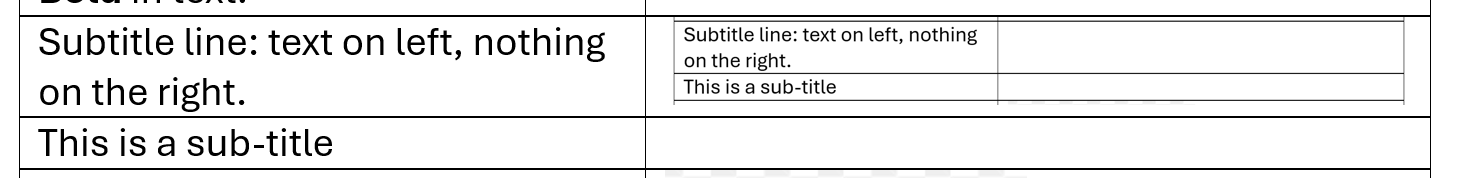
\includegraphics[width=\linewidth,height=0.3\textheight,keepaspectratio]{./Resources/figure_generated/2.png}}
\end{minipage}\\ \hline


\multicolumn{3}{|c|}{%
    \begin{minipage}{\linewidth}
        \centering
        \vspace{0.5em}\Large This is a sub-title\vspace{0.5em}
    \end{minipage}
}\\ \hline          


\centering \steplist
&
Multi images line: text on left, all images on the right. Keep all images in the same line in the table.
&
\begin{minipage}[b]{\linewidth}
    \centering
    \raisebox{-.5\height}{
\includegraphics[width=\linewidth,height=0.3\textheight,keepaspectratio]{./Resources/figure_generated/3.png}}
\end{minipage}\\ \hline


\centering 
&
(Continued Image)
&
\begin{minipage}[b]{\linewidth}
    \centering
    \raisebox{-.5\height}{
\includegraphics[width=\linewidth,height=0.3\textheight,keepaspectratio]{./Resources/figure_generated/4.png}}
\end{minipage}\\ \hline


\centering 
&
(Continued Image)
&
\begin{minipage}[b]{\linewidth}
    \centering
    \raisebox{-.5\height}{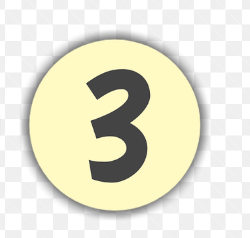
\includegraphics[width=\linewidth,height=0.3\textheight,keepaspectratio]{./Resources/figure_generated/5.png}}
\end{minipage}\\ \hline

\end{longtable}
